\section{El elemento en su posición}

La implementación de todos los algoritmos realizados es de la forma:
\begin{description}
 \item[Entrada:] Vector \texttt{v} y su tamaño \texttt{n}
 \item[Salida:] Entero no negativo que indica el $i$ tal que $v[i]=i$ en caso de que exista o $-1$ en otro caso
\end{description}

En el caso del algoritmo recursivo necesitamos un parámetro adicional para pasar información adicional, pero utilizamos una función \textit{wrapper} que incializa este parámetro adecuadamente.

\subsection{Descripción de los algoritmos y eficiencia teórica}

El algoritmo \textbf{obvio} que resuelve el problema de \textit{El elemento en su posición} consiste
en recorrer cada elemento del vector y comprobar para cada uno de estos si se cumple la
condición deseada ($v[i] = i$):

% Versión obvia
\lstinputlisting[firstline=23, lastline=28]{cpps/posicion.cpp}

Las condiciones de comienzo, actualización y final del bucle son todas $O(1)$, así como el código del interior del bucle. El bucle se ejecutará un máximo de \texttt{n} veces, por lo que es claro que la eficiencia de este algoritmo es de $\mathbf{O(n)}$.

\vspace*{1cm}
\hrulefill
\vspace*{1cm}

Para el algoritmo \textbf{divide y vencerás} hemos realizado dos versiones. La primera de ellas realiza el algoritmo de forma recursiva mientras que la segunda de forma no recursiva. Dada la similitud de nuestro problema con la búsqueda en un vector, nos hemos inspirado en la búsqueda binaria para realizar el siguiente algoritmo:

% Versión recursiva
\lstinputlisting[firstline=39, lastline=62]{cpps/posicion.cpp}

%% TODO: Explicación del algoritmo
%% TODO: Párrafo sobre la eficiencia de la versión recursiva

La versión no recursiva, basada en la versión no recursiva de la búsqueda binaria queda:

% Versión no recursiva
\lstinputlisting[firstline=76, lastline=77]{cpps/posicion.cpp}

%% TODO: Explicación y comparación del algoritmo
%% TODO: Párrafo sobre la eficiencia de la versión no recursiva

\subsection{Determinación del umbral}

En el caso del algoritmo divide y vencerás hemos hecho un estudio del mismo para determinar el umbral para el caso base (para el cual utilizamos el algoritmo obvio) que resulta más eficiente.

%% TODO: Antonio escribe aquí

\begin{figure}[H]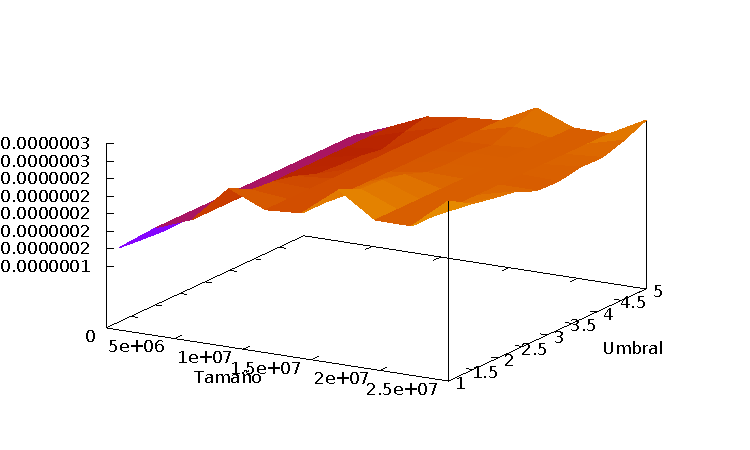
\includegraphics[width=13cm]{img/umbral_posicion.pdf} \centering
	\caption{Tiempos según Umbral y Tamaño}\end{figure}

\subsection{Eficiencia empírica de los algoritmos}

Utilizando la librería \texttt{chrono} hemos medido los tiempos de los algoritmos para un conjunto fijo de tamaños. Aunque los algoritmos son rápidos para tamaños grandes, las funciones auxiliares utilizadas para la generación de muestras aleatorias que permitan medir el tiempo han dificultado la obtención de los datos. Los datos obtenidos pueden verse en la siguiente tabla:

% tex.stackexchange.com/questions/10284

\vspace*{1cm}

\pgfplotstableread{dats/comp_umbral_posicion/posicion_t.dat}\posObvio
\pgfplotstableread{dats/comp_umbral_posicion/posicion_1.dat}\posDyV
%\pgfplotstableread{dats/comp_umbral_posicion/posicion_2.dat}\posDyVTwo
\pgfplotstablecreatecol[copy column from table={\posDyV}{[index] 1}] {par1} {\posObvio}
%\pgfplotstablecreatecol[copy column from table={\posDyVTwo}{[index] 1}] {par2} {\posObvio}

\pgfplotstabletypeset[
display columns/0/.style={column name=Tamaño},
display columns/1/.style={column name=Algoritmo Obvio},
display columns/2/.style={column name=Algoritmo DyV (r)},
skip rows between index={25}{50}
%display columns/3/.style={column name=Algoritmo DyV (no recursivo)},
]{\posObvio}

\vspace*{1cm}

Podemos ajustar estos datos con una función representativa del orden de eficiencia teórico obtenido en la sección anterior:

%% TODO: Ajustes de las funciones

En el siguiente gráfico podemos observar además una comparativa de las eficiencias empíricas y teóricas de los algoritmos realizados:

%% TODO: Gráfica con todos los algoritmos

\subsection{Vectores con elementos repetidos}
